\documentclass[a4paper, 14pt]{article}
\usepackage[margin=2.25cm]{geometry}
\usepackage[utf8]{inputenc}
\usepackage{minted}
\usepackage[russian]{babel}
\usepackage{amsmath}
\usepackage{graphicx}
\usepackage{changepage}
\usepackage{hyperref}
\usepackage{cases}
\usepackage{indentfirst}
\usepackage{multirow}
\usepackage{longtable}
\pagestyle{plain}

\hypersetup{
	linkbordercolor = {1 1 1}
}

\usepackage[usenames,dvipsnames,svgnames,table]{xcolor}
\usepackage{tikz-timing}[2009/05/15]
\usepackage{multicol}
\usepackage[T2A]{fontenc}
\usepackage{pgfplots}
\usepackage{pgfgantt}

\usepackage{listings}
\usepackage{caption}
\DeclareCaptionFont{white}{\color{white}} % Текст заголовка.
\DeclareCaptionFormat{listing}{\colorbox{gray}{\parbox{\textwidth}{#1#2#3}}}
\captionsetup[lstlisting]{format=listing,labelfont=white,textfont=white}
\renewcommand\labelenumi{\theenumi)}

\usepackage[backend=biber]{biblatex}
\addbibresource{mybib.bib}

\def\Year{\expandafter\YEAR\the\year}
\def\YEAR#1#2#3#4{#1#2#3#4}



\begin{document}
\lstset{
	language=java,                 % Выбор языка для подсветки (здесь это java).
	basicstyle=\small\sffamily,    % Размер и начертание шрифта для подсветки кода.
	numbers=left,                  % Где поставить нумерацию строк (слева\справа).
	numberstyle=\tiny,             % Размер шрифта для номеров строк.
	stepnumber=1,                  % Размер шага между двумя номерами строк.
	firstnumber=1,
	numberfirstline=true
	numbersep=5pt,                 % Как далеко отстоят номера строк от подсвечиваемого кода.
	backgroundcolor=\color{white}, % Цвет фона подсветки - используем \usepackage{color}.
	showspaces=false,              % Показывать или нет пробелы специальными отступами.
	showstringspaces=false,        % Показывать или нет пробелы в строках.
	showtabs=false,                % Показывать или нет табуляцию в строках.
	frame=single,                  % Рисовать рамку вокруг кода.
	tabsize=2,                     % Размер табуляции по умолчанию равен 2 пробелам.
	captionpos=t,                  % Позиция заголовка вверху [t] или внизу [b].
	breaklines=true,               % Автоматически переносить строки (да\нет).
	breakatwhitespace=false,       % Переносить строки только если есть пробел.
	escapeinside={\%*}{*)}         % Если нужно добавить комментарии в коде.
}

\begin{titlepage}
	\center
	МИНИСТЕРСТВО НАУКИ И ВЫСШЕГО ОБРАЗОВАНИЯ РОССИЙСКОЙ ФЕДЕРАЦИИ\linebreak
	ФЕДЕРАЛЬНОЕ ГОСУДАРСТВЕННОЕ АВТОНОМНОЕ ОБРАЗОВАТЕЛЬНОЕ УЧРЕЖДЕНИЕ ВЫСШЕГО ОБРАЗОВАНИЯ\linebreak
	Национальный исследовательский ядерный университет <<МИФИ>> (НИЯУ МИФИ)
	\noindent\rule{500pt}{0.8pt} \\
	\textsc{\Large Институт интеллектуальных кибернетических систем}\\[8.5cm]

	{ \huge \bfseries ОТЧЕТ ПО ИТОГОВОМУ ПРОЕКТУ	\\
	\Large \mdseries СЕРВИС КОРОТКИХ ССЫЛОК \\
	\large по дисциплине <<Программирование на языке Java>>}\\[7.0cm]


	\begin{multicols}{2}
		\begin{flushright} \large

			{Выполнил студент группы: М24-535:}\\[0.5cm]

			{Преподаватели:\\}

		\end{flushright}
		\begin{flushright}

			{Почернин В. С.}\\[0.5cm]


			Калин А.\\
			Павлюк Г.

		\end{flushright}
	\end{multicols}

	\flushright{
		{\today}\\[0.5cm]
	}
	\centering{
		Санкт-Петербург\\
		\Year
	}

	\vfill
\end{titlepage}

\large
\tableofcontents

\newpage
\section{Описание проекта}

Сервис коротких ссылок представляет собой \texttt{Java} приложение с консольным интерфейсом, позволяющее различным пользователем создавать, редактировать и использовать короткие ссылки.

Сервис написан в строгом соответствии с критериями, описанными в \texttt{README.md} (соответствие критериям будет показано ниже).

\subsection{Используемые технологии}

\begin{itemize}
	\item \texttt{Java} - язык программирования.
	\item \texttt{Spring} - основной фреймворк.
	\item \texttt{PostgreSQL} - используемая СУБД.
	\item \texttt{Maven} - система сборки проекта.
	\item \texttt{Flyway} - инструмент для применения файлов миграций БД.
	\item \texttt{Lombok} - библиотека для сокращения шаблонного кода.
\end{itemize}

\subsection{Описание модулей}

Вкратце рассмотрим кодовую базу проекта:

\begin{itemize}
	\item Пакет \texttt{command}: содержит в себе классы, отвечающие за работу интерфейса командной строки, такие как сама команда, типы команд, а также сам класс интерфейса.
	\item Пакет \texttt{context}: содержит класс, отвечающий за переменные контекста сервиса.
	\item Пакет \texttt{entity}: содержит классы моделей данных (связанных с базой при помощи \texttt{ORM}).
	\item Пакет \texttt{exception}: содержит в себе класс-исключение, связанное с сервисом коротких ссылок.
	\item Пакет \texttt{handler}: содержит в себе классы, реализующие паттерн <<стратегия>> и используемые для обработки команд.
	\item Пакет \texttt{repository}: содержит в себе классы - \texttt{JPA} репозитории.
	\item Пакет \texttt{utils}: содержит в себе различные утильные классы.
	\item Папка \texttt{migration}: содержит в себе файлы миграции БД, которые устанавливают схему и наполняют базу тестовыми данными.
\end{itemize}

\subsection{Схема БД}

База данных проекта имеет следующую схему:

\begin{figure}[H]
	\centering
	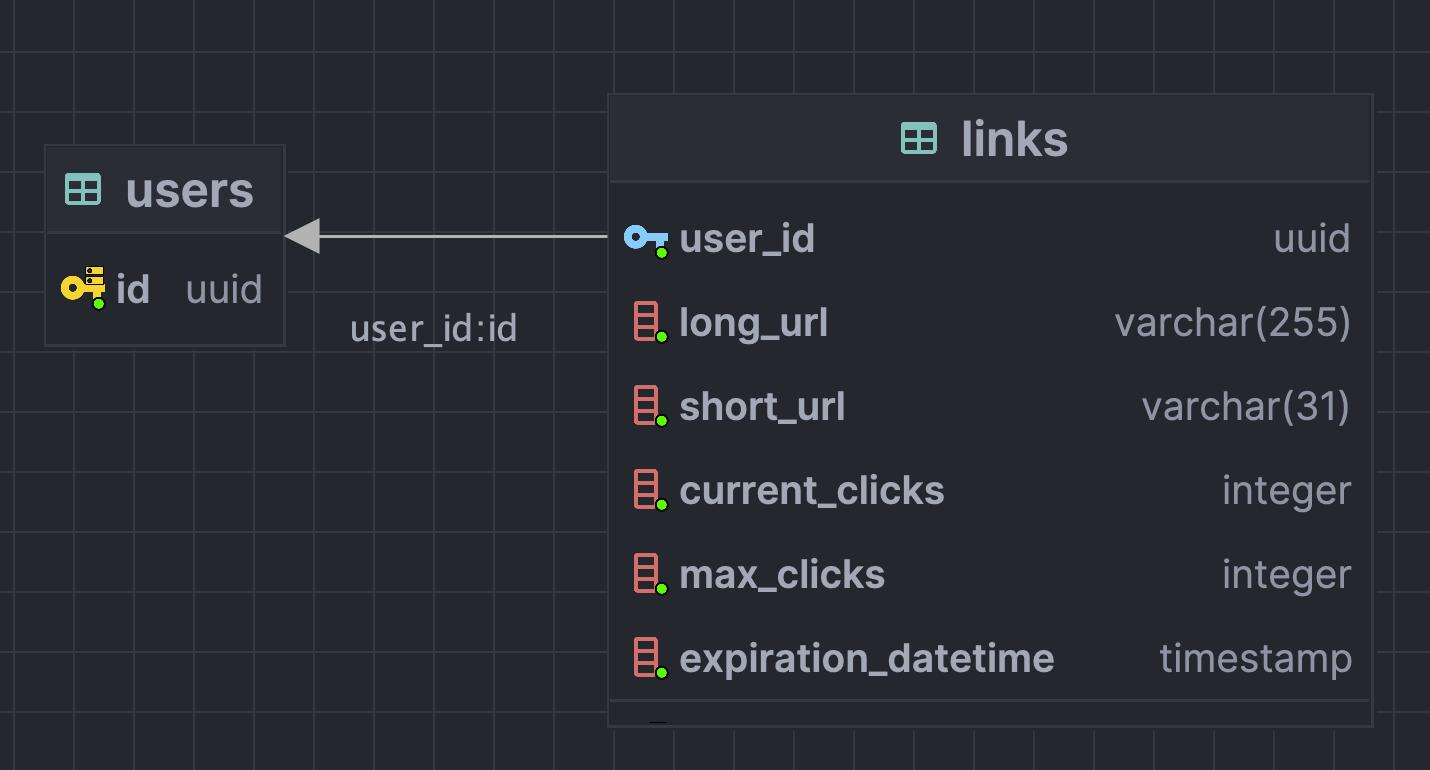
\includegraphics[width=17cm]{resources/3.png}
	\caption{Схема БД}
\end{figure}

Пользователь идентифицируется по \texttt{UUID}.

Каждая ссылка хранит в себе внешний ключ пользователя, длинную ссылку, короткую ссылку, текущее количество кликов, максимальное количество кликов, а также метку времени, когда ссылка перестанет действовать.

На короткую ссылку наложен индекс \texttt{UNIQUE}, что позволяет быстро искать запись по короткой ссылке и предотвращает возможные ошибки.

Также в базу данных автоматически записываются тестовые данные:

\begin{figure}[H]
	\centering
	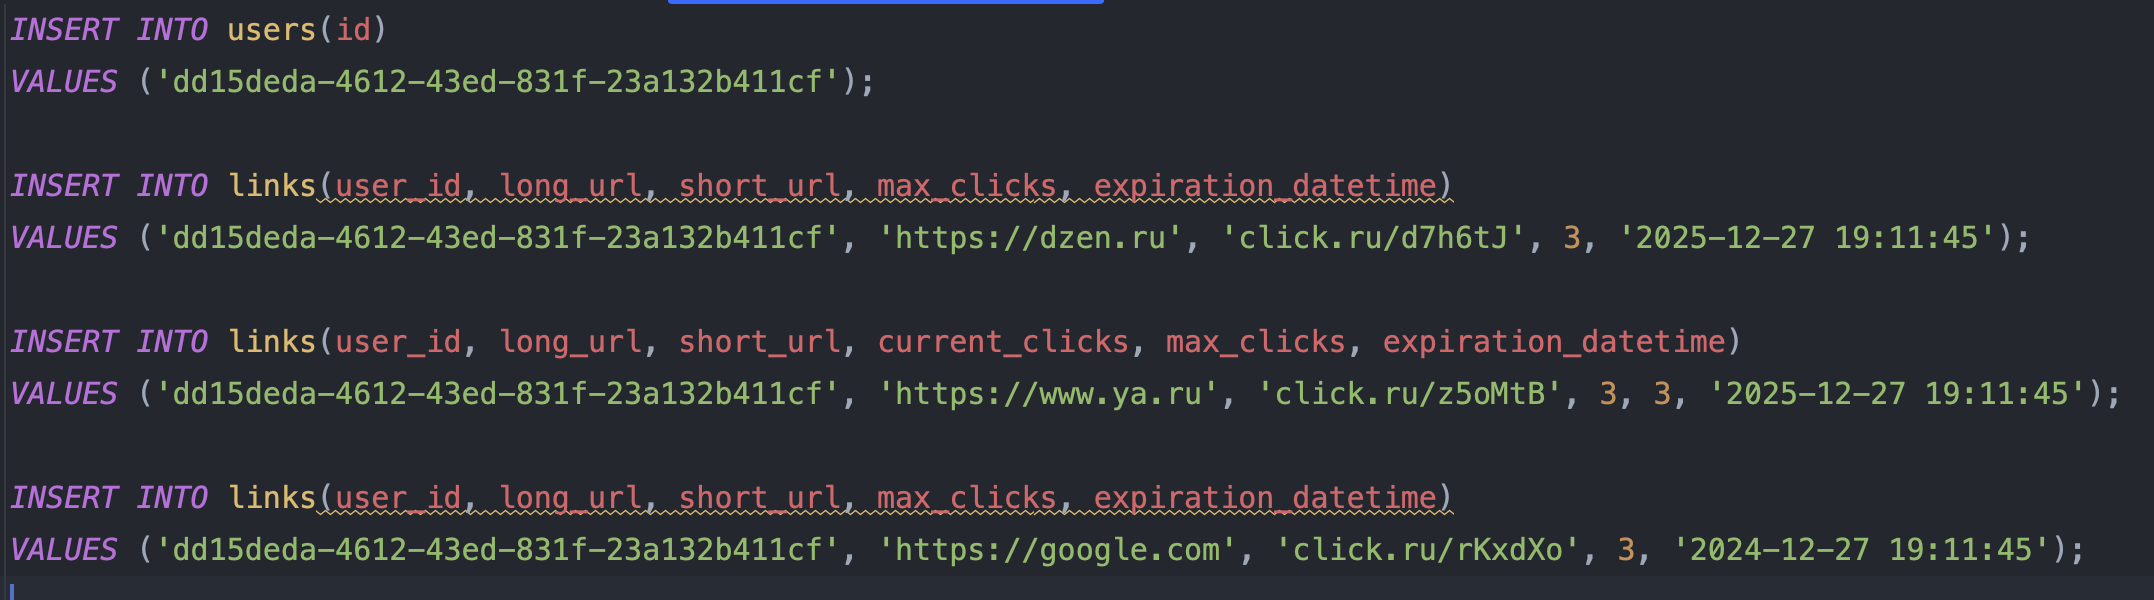
\includegraphics[width=17cm]{resources/4.png}
	\caption{Тестовые данные}
\end{figure}

Пользователь с \texttt {UUID} - \texttt{dd15deda-4612-43ed-831f-23a132b411cf}, а также три ссылки:


\begin{itemize}
	\item \texttt{click.ru/d7h6tJ} - действует;
	\item \texttt{click.ru/z5oMtB} - использована максимальное количество раз;
	\item \texttt{click.ru/rKxdXo} - истек срок действия;
\end{itemize}

\newpage
\section{Инструкции по запуску кода}

Для того, чтобы запустить код, необходимо иметь

\begin{itemize}
	\item \texttt{Java 17} (полагаю, что версии выше также подойдут).
	\item \texttt{Docker} (необходим для быстрого поднятия БД, но можно поднимать руками).
	\item \texttt{Maven} (либо просто запускать проект в \texttt{IntelliJ IDEA}).
\end{itemize}

Запустим наш проект. Для начала, перейдем в директорию, содержащую конфигурационный файл докера - \texttt{/src/main/resources/db}, затем запустим базу данных в \texttt{detach} режиме командой \texttt{docker compose up -d}

\begin{figure}[H]
	\centering
	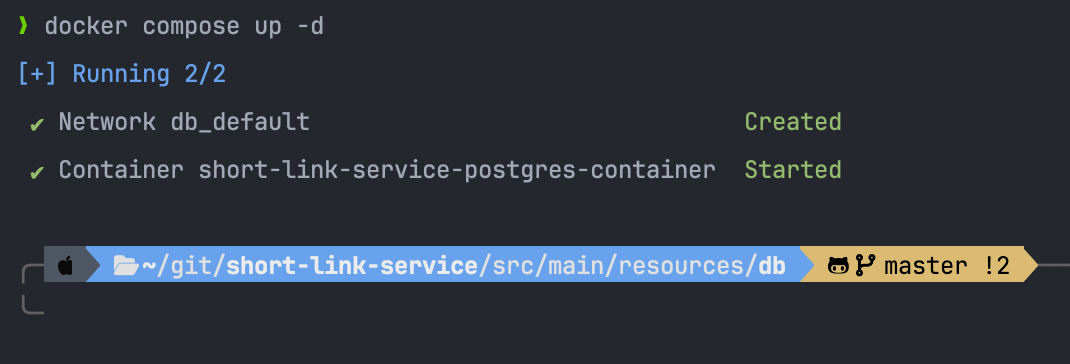
\includegraphics[width=17cm]{resources/1.png}
	\caption{Запуск БД}
\end{figure}

Чтобы собрать проект при использовании \texttt{Maven} вручную, можно написать команду \texttt{mvn clean compile}.

Чтобы запустить сам проект, можно либо сделать это в консоли с помощью \texttt{Maven}, написав команду
\begin{verbatim}
mvn exec:java -Dexec.mainClass=
"ru.vspochernin.short_link_service.ShortLinkServiceApplication"
\end{verbatim}
Либо просто запустить \texttt{main()} метод из класса \texttt{ShortLinkServiceApplication} с помощью \texttt{IntelliJ IDEA} (идея при запуске проекта должна автоматически скачать все зависимости).


После запуска кода, мы увидим приветственное сообщение с описанием всех команд, требованиям к конфигурационному файлу и параметрам.


\begin{figure}[H]
	\centering
	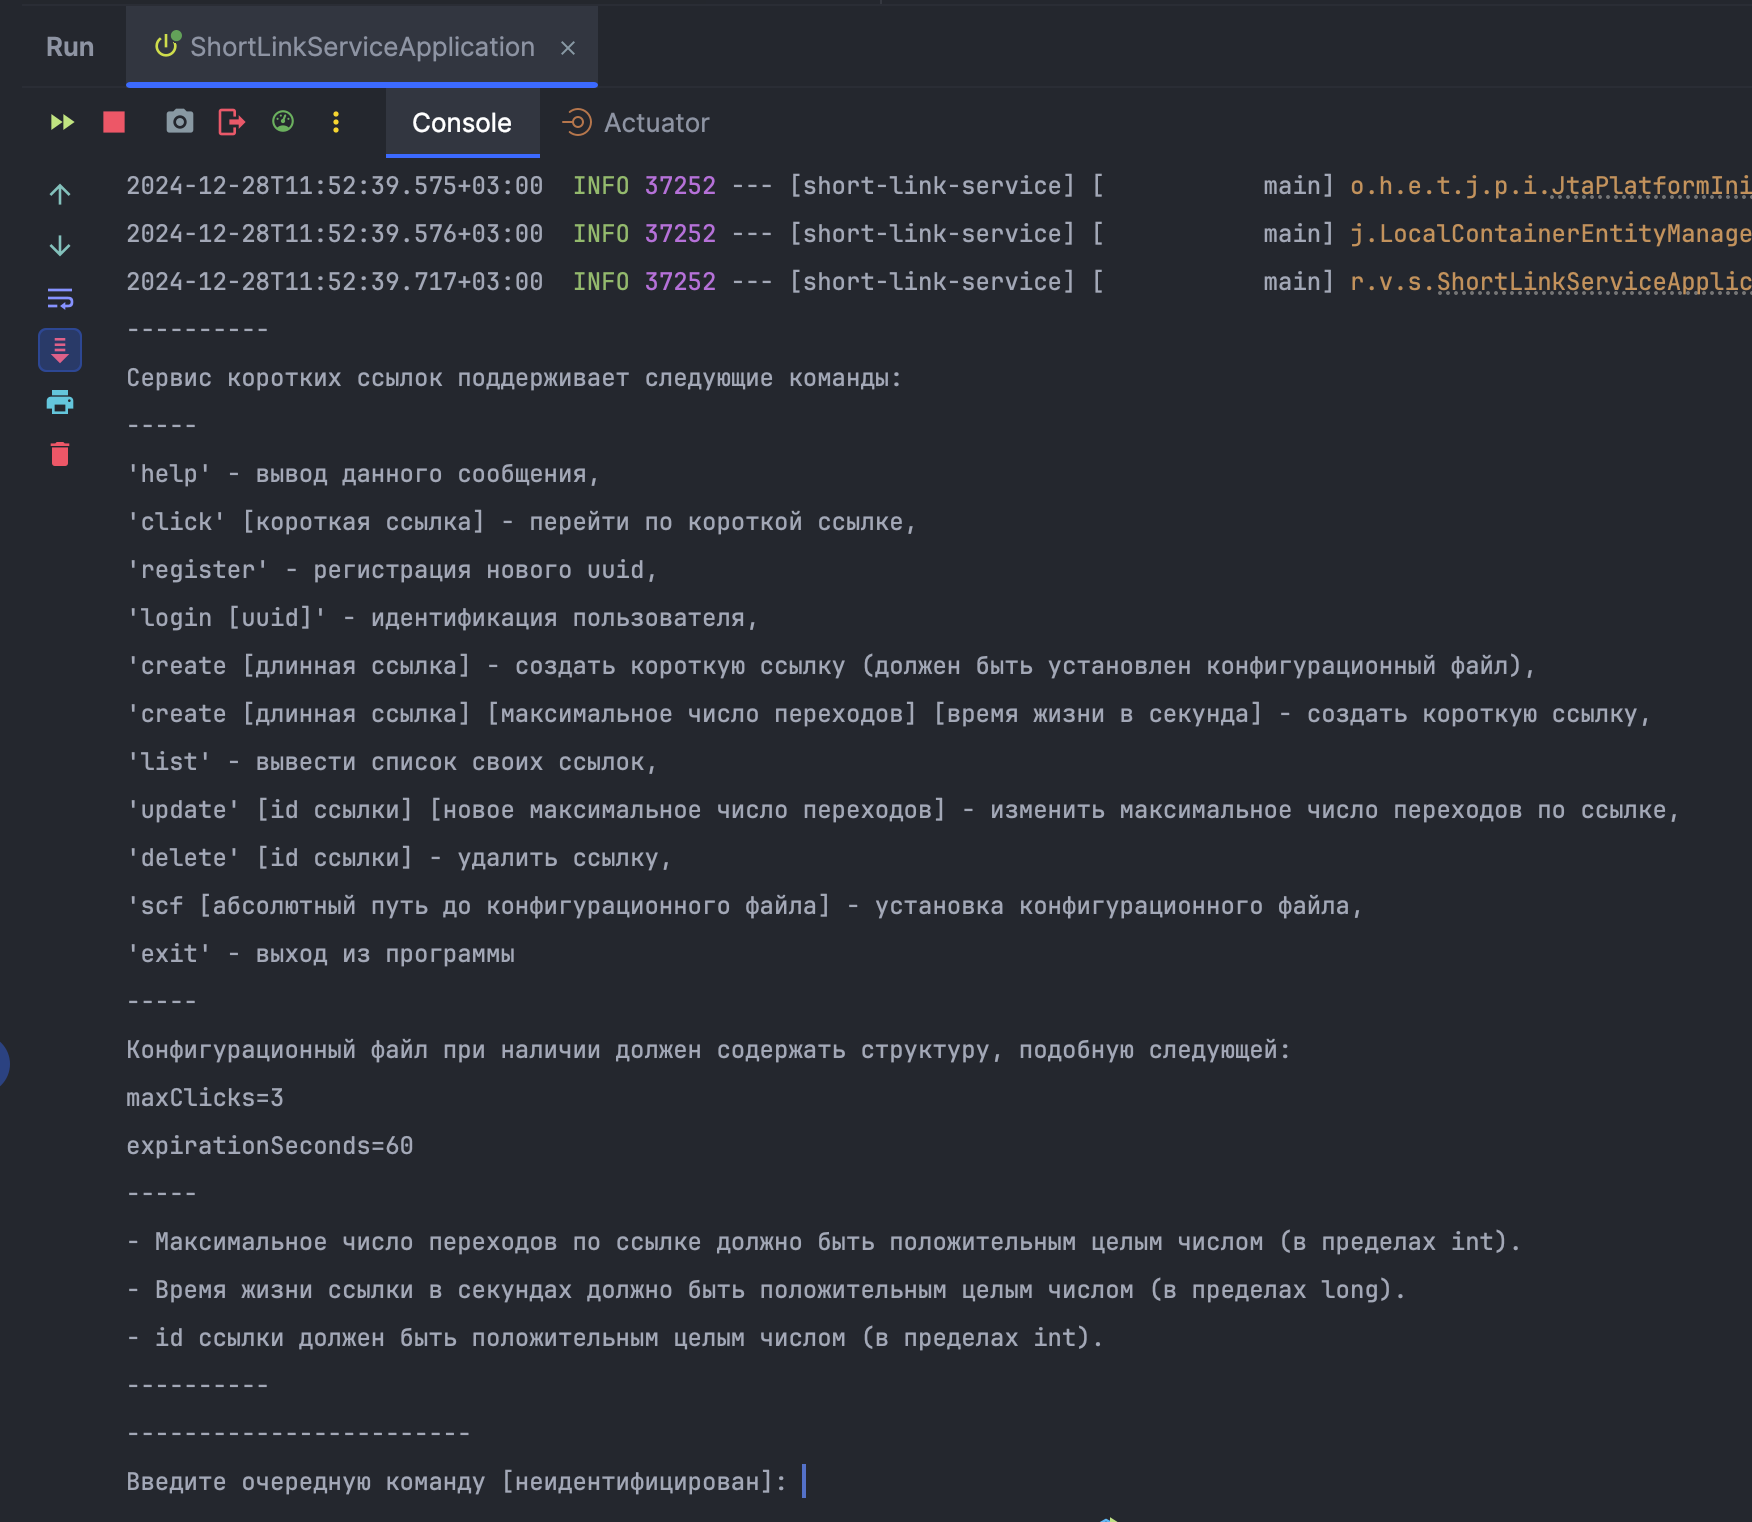
\includegraphics[width=17cm]{resources/2.png}
	\caption{Запуск кода}
\end{figure}

\newpage
\section{Тестирование на соответствие критериям}

Ниже мы пройдемся по каждому критерию и проверим корректность его выполнения.

\subsection{Функциональность}

Алгоритм сокращения ссылки должен корректно работать и возвращать уникальную короткую ссылку для каждого пользователя.

\subsection{Внесение основных параметров работы алгоритма в конфигурационный файл}

При добавлении ссылки пользователь может указать время существования ссылки. Фактическое время хранения должно быть ограничено меньшим из введенных пользователем значений или значений, заданных в конфигурационном файле. Необходимо реализовать возможность подключения конфигурации из отдельного файла

\subsection{Ограничение по времени жизни}

Реализована функция автоматического удаления ссылки по истечении ее срока действия.

\subsection{Автоматическое удаление ссылок}

Ссылки удаляются по достижении лимита переходов или истечения времени жизни.

\subsection{Уникальность ссылок}

Разные пользователи получают разные короткие ссылки на один и тот же \texttt{URL}:

\subsection{Повторное создание ссылки}

При повторном запросе сокращения той же ссылки, пользователю должна быть сгенерирована новая ссылка:

\subsection{Переход по ссылке}

При вводе короткой ссылки в консоль должен осуществляться переход на оригинальный ресурс:

\subsection{Лимит переходов}

Ссылка должна блокироваться после достижения заданного пользователем лимита переходов. Пользователь вводит этот лимит и, в зависимости от заданного времени существования ссылки, система выбирает большее из введенного пользователем значения и значения, заданного в конфигурационном файле.

\subsection{Уведомление пользователя}

Пользователь получает уведомление, когда ссылка становится недоступной из-за лимита переходов или истечения времени жизни.

\subsection{Редактирование лимита переходов}

У пользователя есть возможность изменять лимит переходов по ссылке.

\subsection{Удаление ссылки}

Пользователь может удалять свои ссылки.

\subsection{Идентификация по UUID}

Возможность редактирования и удаления ссылки должна быть доступна только ее создателю, идентифицируемому по \texttt{UUID}.

\subsection{Работа нескольких пользователей}

Сервис поддерживает работу нескольких пользователей, каждый из которых может создавать уникальные короткие ссылки.

\subsection{Администрирование параметров ссылки}

Только создатель ссылки может редактировать ее параметры или удалять ее.

\subsection{Создание нескольких ссылок}

Один пользователь может создавать несколько коротких ссылок на разные ресурсы.

\subsection{Идентификация по UUID при повторных запросах}

Система идентифицирует пользователя по \texttt{UUID} и генерирует уникальную ссылку при каждом запросе

\end{document}